\chapter[Keynotes]{Keynotes}

\section{Monday, July 28}


\begin{center}
    {\Large \textbf{Rethinking Pretraining: Data and Architecture}}
    
    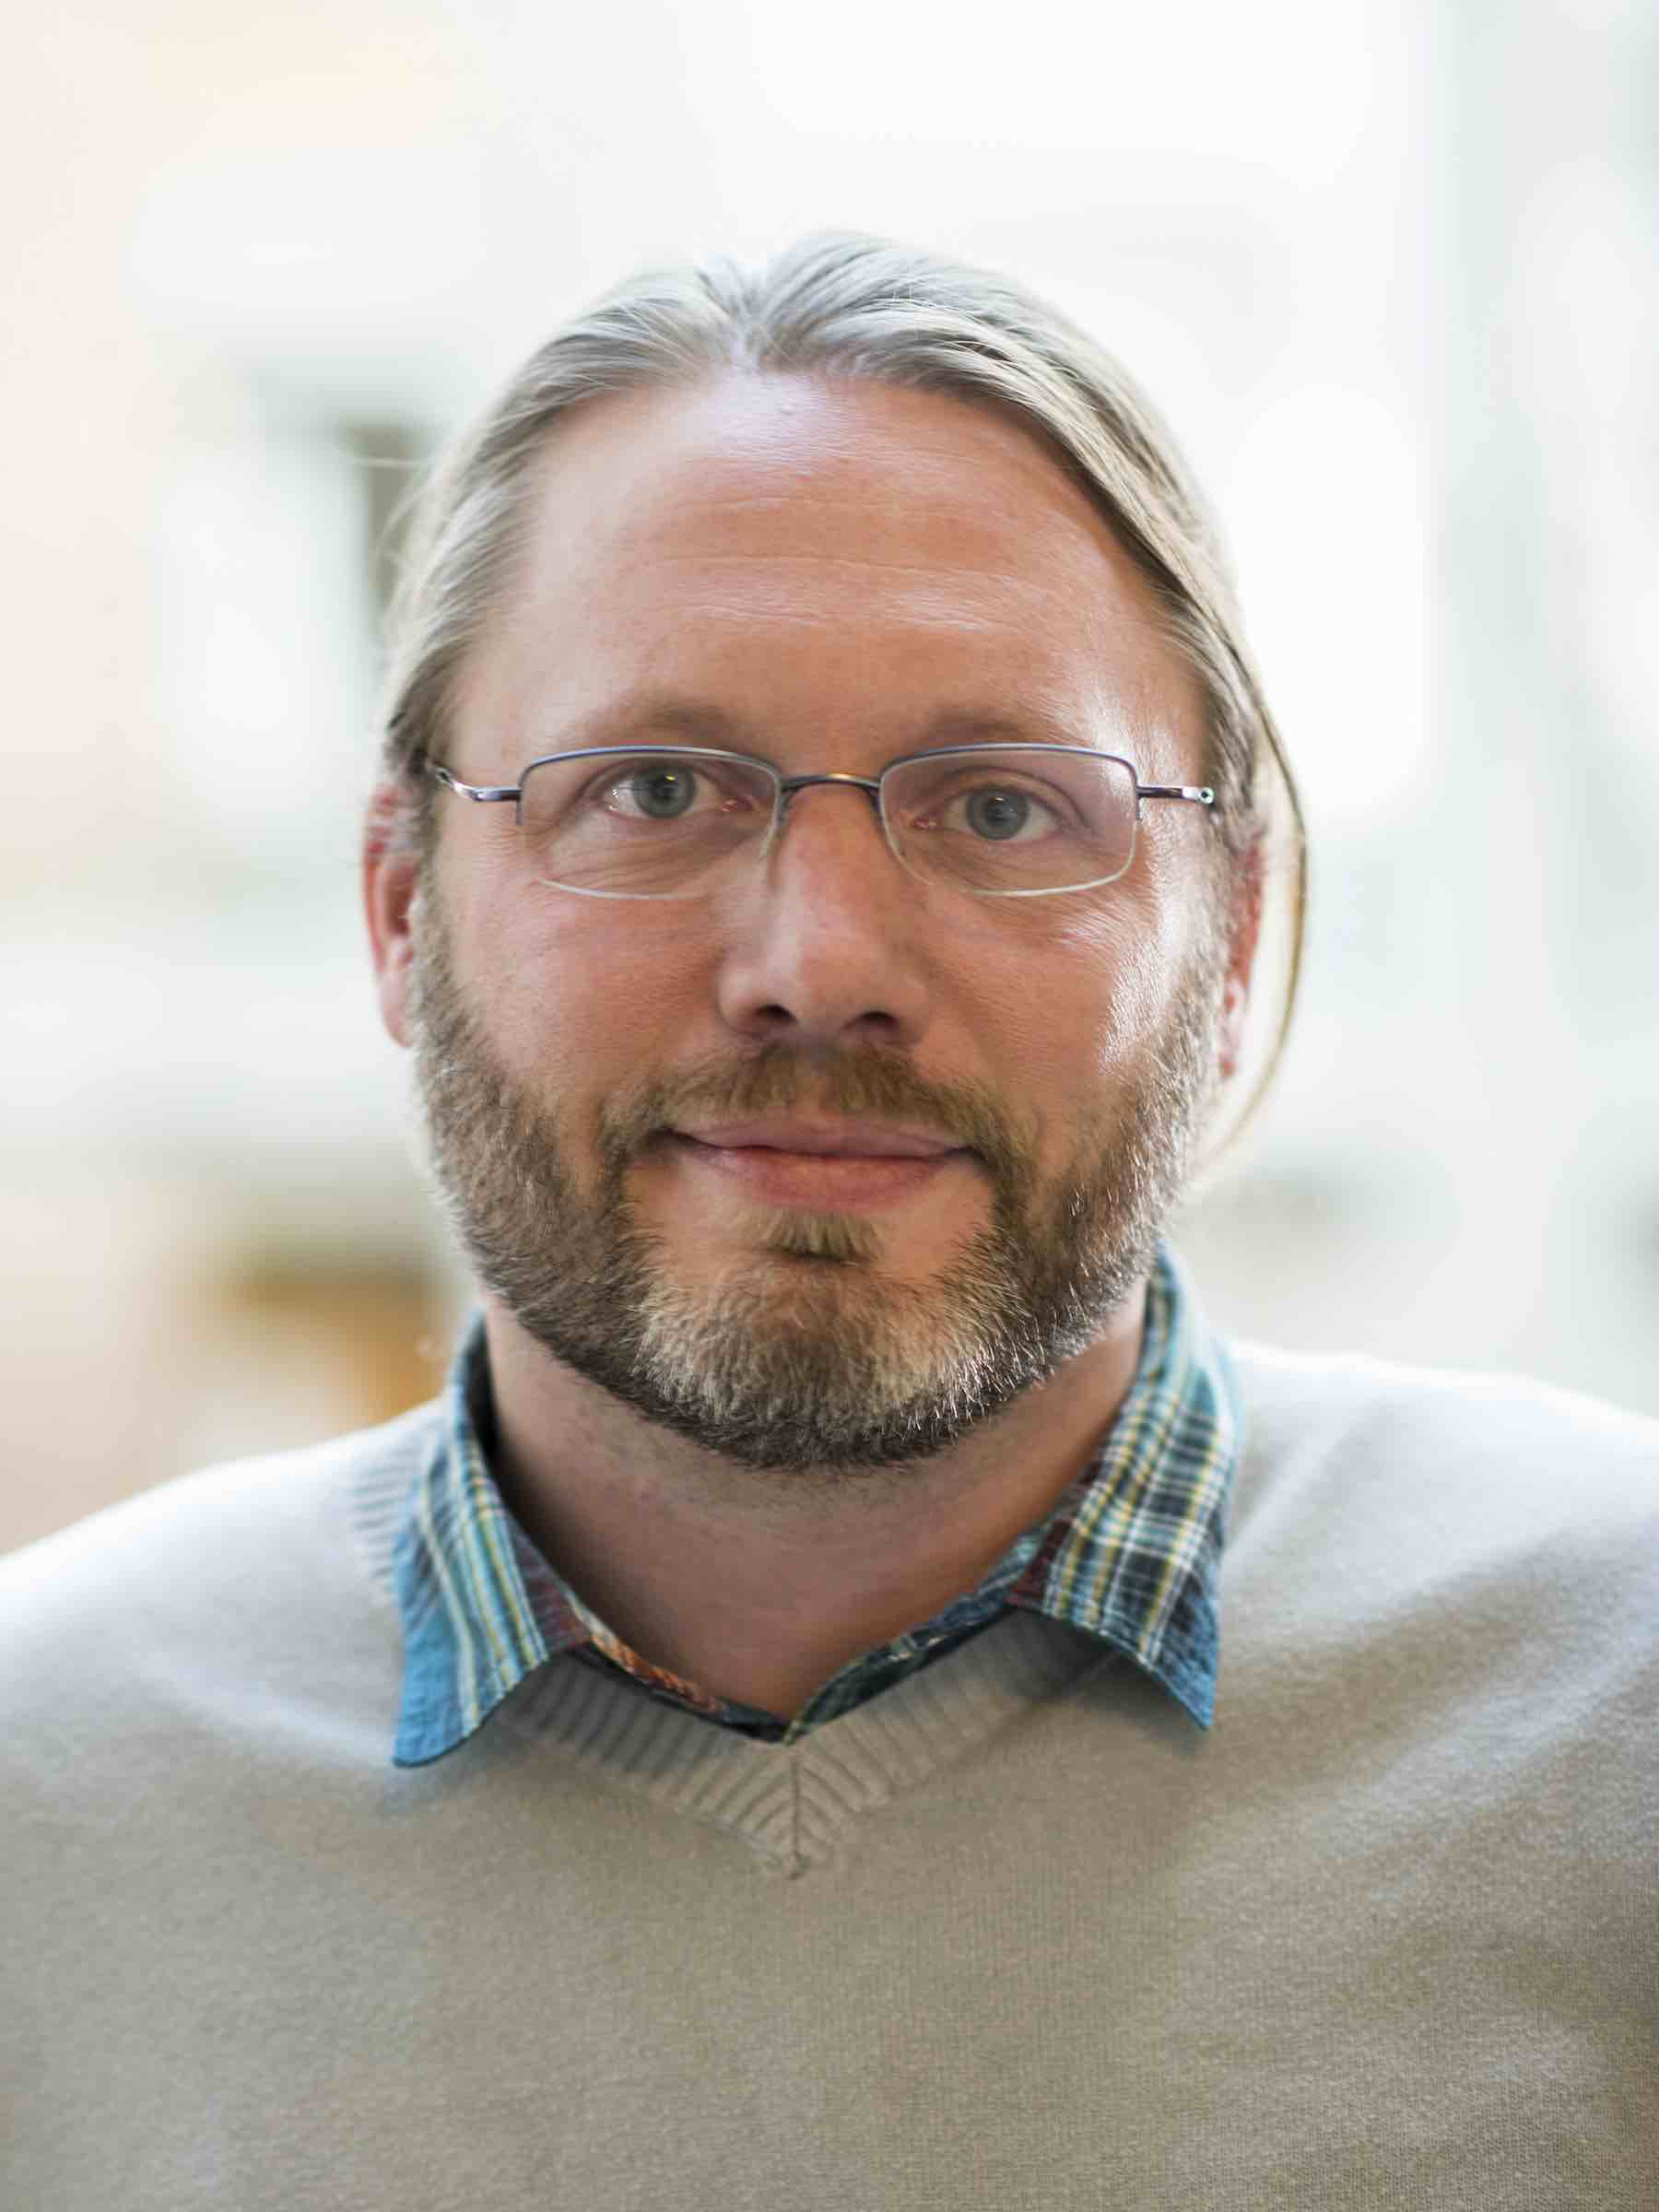
\includegraphics[width=1.5in]{luke.jpg}
    
    {\large \textbf{Luke Zettlemoyer}}

    Monday, July 28, 09:30 - 10:30
\end{center}

\paragraph{Abstract:}
Large language model training follows a standard pipeline: tokenization, pretraining, possibly mid-training, and post training or alignment. Despite its wild success, we understand relatively little about this recipe and are almost certainly missing many opportunities to improve it. In this talk, I will focus on three such cases. I’ll describe our work on data efficient post training (e.g. LIMA, ALMA, and s1) where we argue that nearly all advanced model capabilities ultimately come from the pretraining data, even if effective alignment is still essential for controlling model behavior. I will also describe new methods for extracting more signal from the pretraining data, including new hierarchical architectures for byte-level language models (e.g. BLT) that are both tokenizer-free and scale better than traditional BPE-based methods, especially in the long tail. Finally, I will discuss decentralized, modular training algorithms (e.g. BTM) that better isolate and control the influence of specific data on specific model components and behaviors. Together, these methods promise to simplify training and improve scaling, by centering and amplifying the influence of data in architecture design. 

\paragraph{Bio:}
Luke Zettlemoyer is a Professor in the Paul G. Allen School of Computer Science & Engineering at the University of Washington, and a Senior Research Director at Meta. His research focuses on empirical methods for natural language semantics, and involves designing machine learning algorithms, introducing new tasks and datasets, and, most recently, studying how to best develop new architectures and self-supervision signals for pre-training. His honors include being elected ACL President, named an ACL Fellow, winning a PECASE award, an Allen Distinguished Investigator award, and multiple best paper awards. Luke was an undergrad at NC State, received his PhD from MIT and was a postdoc at the University of Edinburgh.

\index{Zettlemoyer!Luke}

\clearpage


\section{Tuesday, July 29}


\begin{center}
    {\Large \textbf{Whose Gold? Re-imagining Alignment for Truly Beneficial AI}}
    
    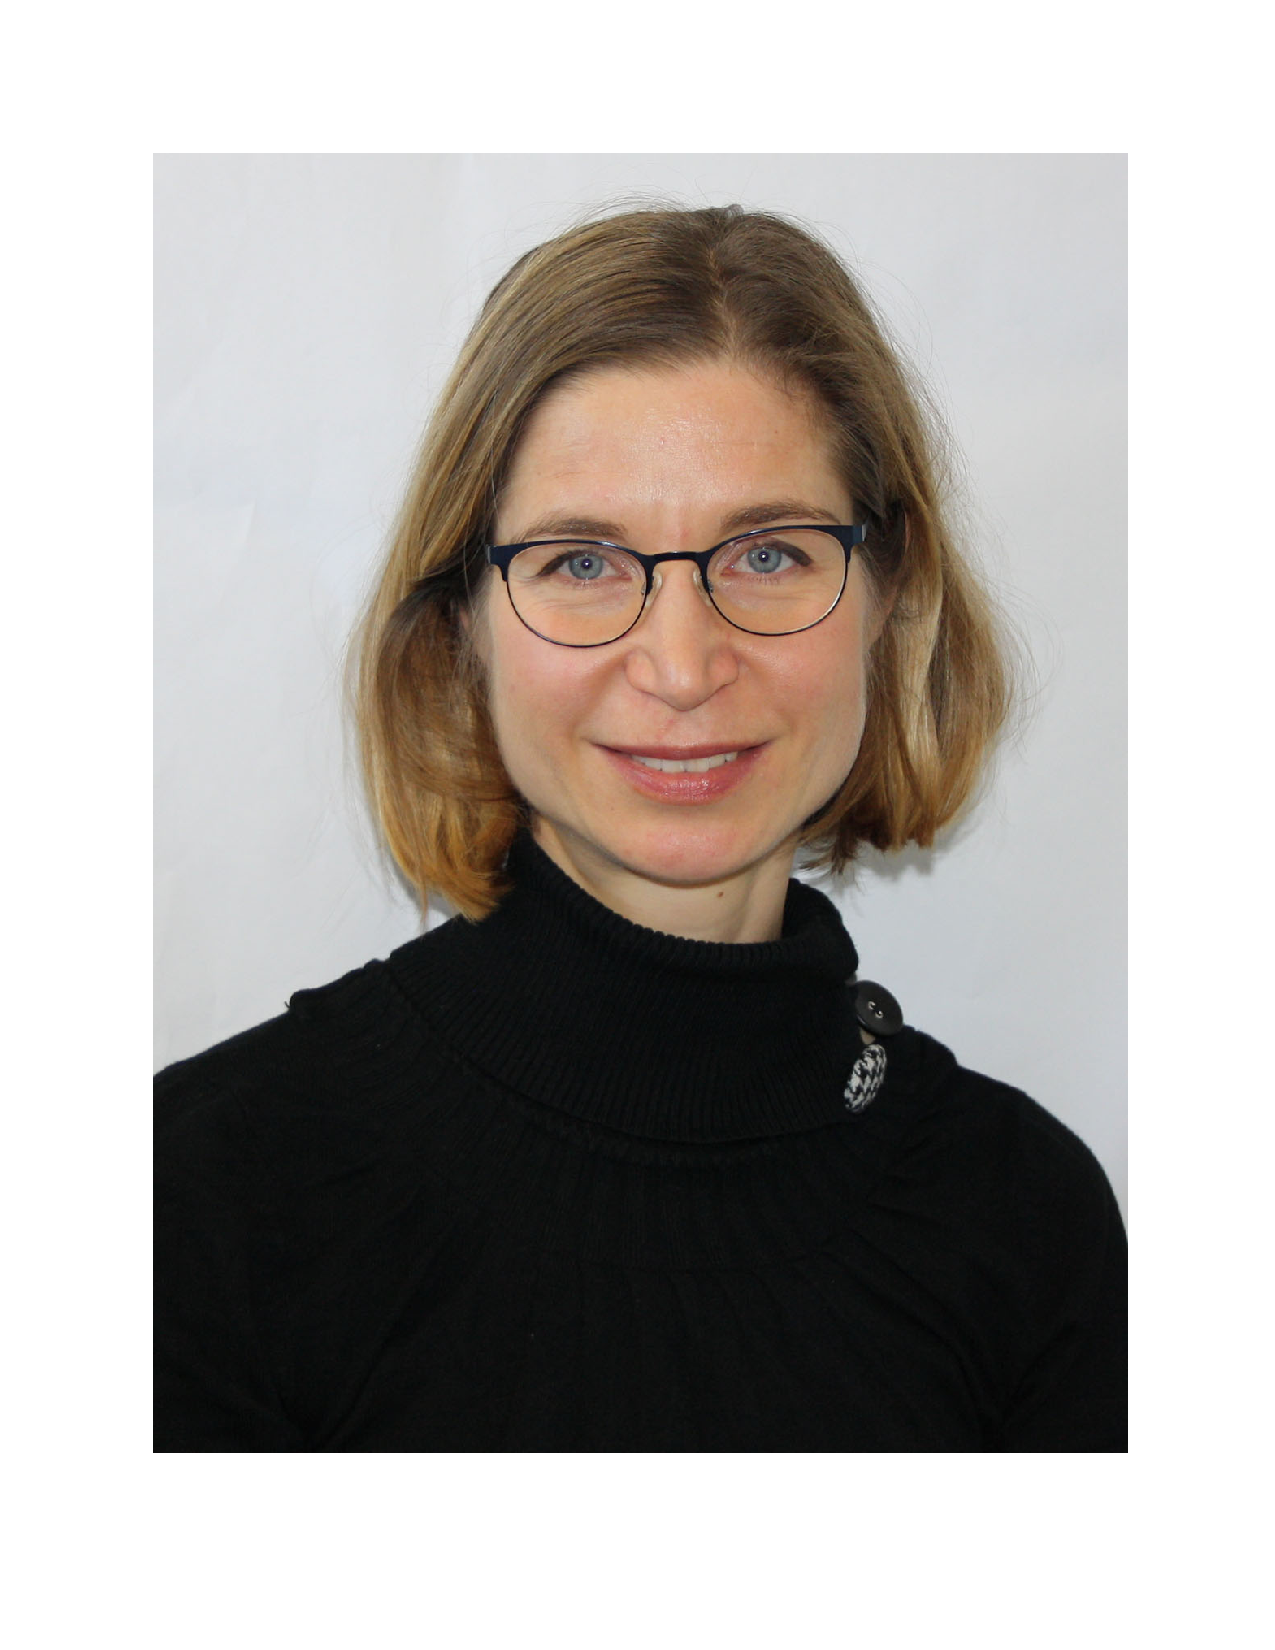
\includegraphics[width=1.5in]{Verena.pdf}
    
    {\large \textbf{Verena Rieser}}

    Monday, July 28, 09:00 - 10:00
\end{center}

\paragraph{Abstract:}
Human feedback is often the "gold standard" for AI alignment, but what if this "gold" reflects diverse, even contradictory human values? This keynote explores the technical and ethical challenges of building beneficial AI when values conflict -- not just between individuals, but also within them. My talk advocates for a dual expansion of the AI alignment framework: moving beyond a single, monolithic viewpoint to a plurality of perspectives, and transcending narrow safety and engagement metrics to promote comprehensive human well-being. 

\paragraph{Bio:}
Verena Rieser is a Senior Staff Research Scientist at Google DeepMind, where she founded the VOICES team (Voices-of-all in alignment). Her team is a core contributor to Gemini with a mission to enhance model safety and usability for diverse communities. Verena has pioneered work in data-driven multimodal Dialogue Systems and Natural Language Generation, encompassing conversational RL agents, faithful data-to-text generation, spoken language understanding, evaluation methodologies, and applications of AI for societal good. Verena previously directed the NLP lab as a full professor at Heriot-Watt University, Edinburgh, and held a Royal Society Leverhulme Senior Research Fellowship. She earned her PhD from Saarland University.

\index{Rieser!Verena}
